\section{PointNet Review}

PointNet \cite{DBLP:journals/corr/QiSMG16} 是斯坦福大学的 C.R. Qi 等人提出
的一种新型的神经网络用于处理、学习三维视觉数据——点云。该网络可以用于三维物体的
分类与语义分割。 这种神经网络直接作用于点云数据,几乎不需要经过任何的变化。使用特
征转换与“类卷积”的神经网络处理三维数据空间的特征。

\subsection{数学模型}
  
PointNet 再数学上的目标是建立一个神经网络用于近似公式 \eqref{eq:mathmodel}
\begin{equation}
  \label{eq:mathmodel}
  f\left( \left\{ x_1,\dots, x_n \right\} \right) \approx g\left( h(x_1),\dots, h(x_n) \right)
\end{equation}
其中有 $f : 2^{\mathbb{R}^N} \rightarrow \mathbb{R}$, $h : \mathbb{R}^N
\rightarrow \mathbb{R}^K$ 和 $g :  \underbrace{\mathbb{R}^K \times \cdots \times
  \mathbb{R}^K}_{n} \rightarrow \mathbb{R}$ 是对称函数。


\subsection{网络结构}

PointNet 的网络结构由共享参数的神经网络与特征变换组成。共享参数的神经网络实质
上是广义卷积神经网络,再在其作者的代码实现中也是使用 TensorFlow 的卷积完成的。特
征变换则是将“传入”信号通过 “T-Net” 之后与其本身进行矩阵乘法得到的。

\begin{figure}
  \centering
  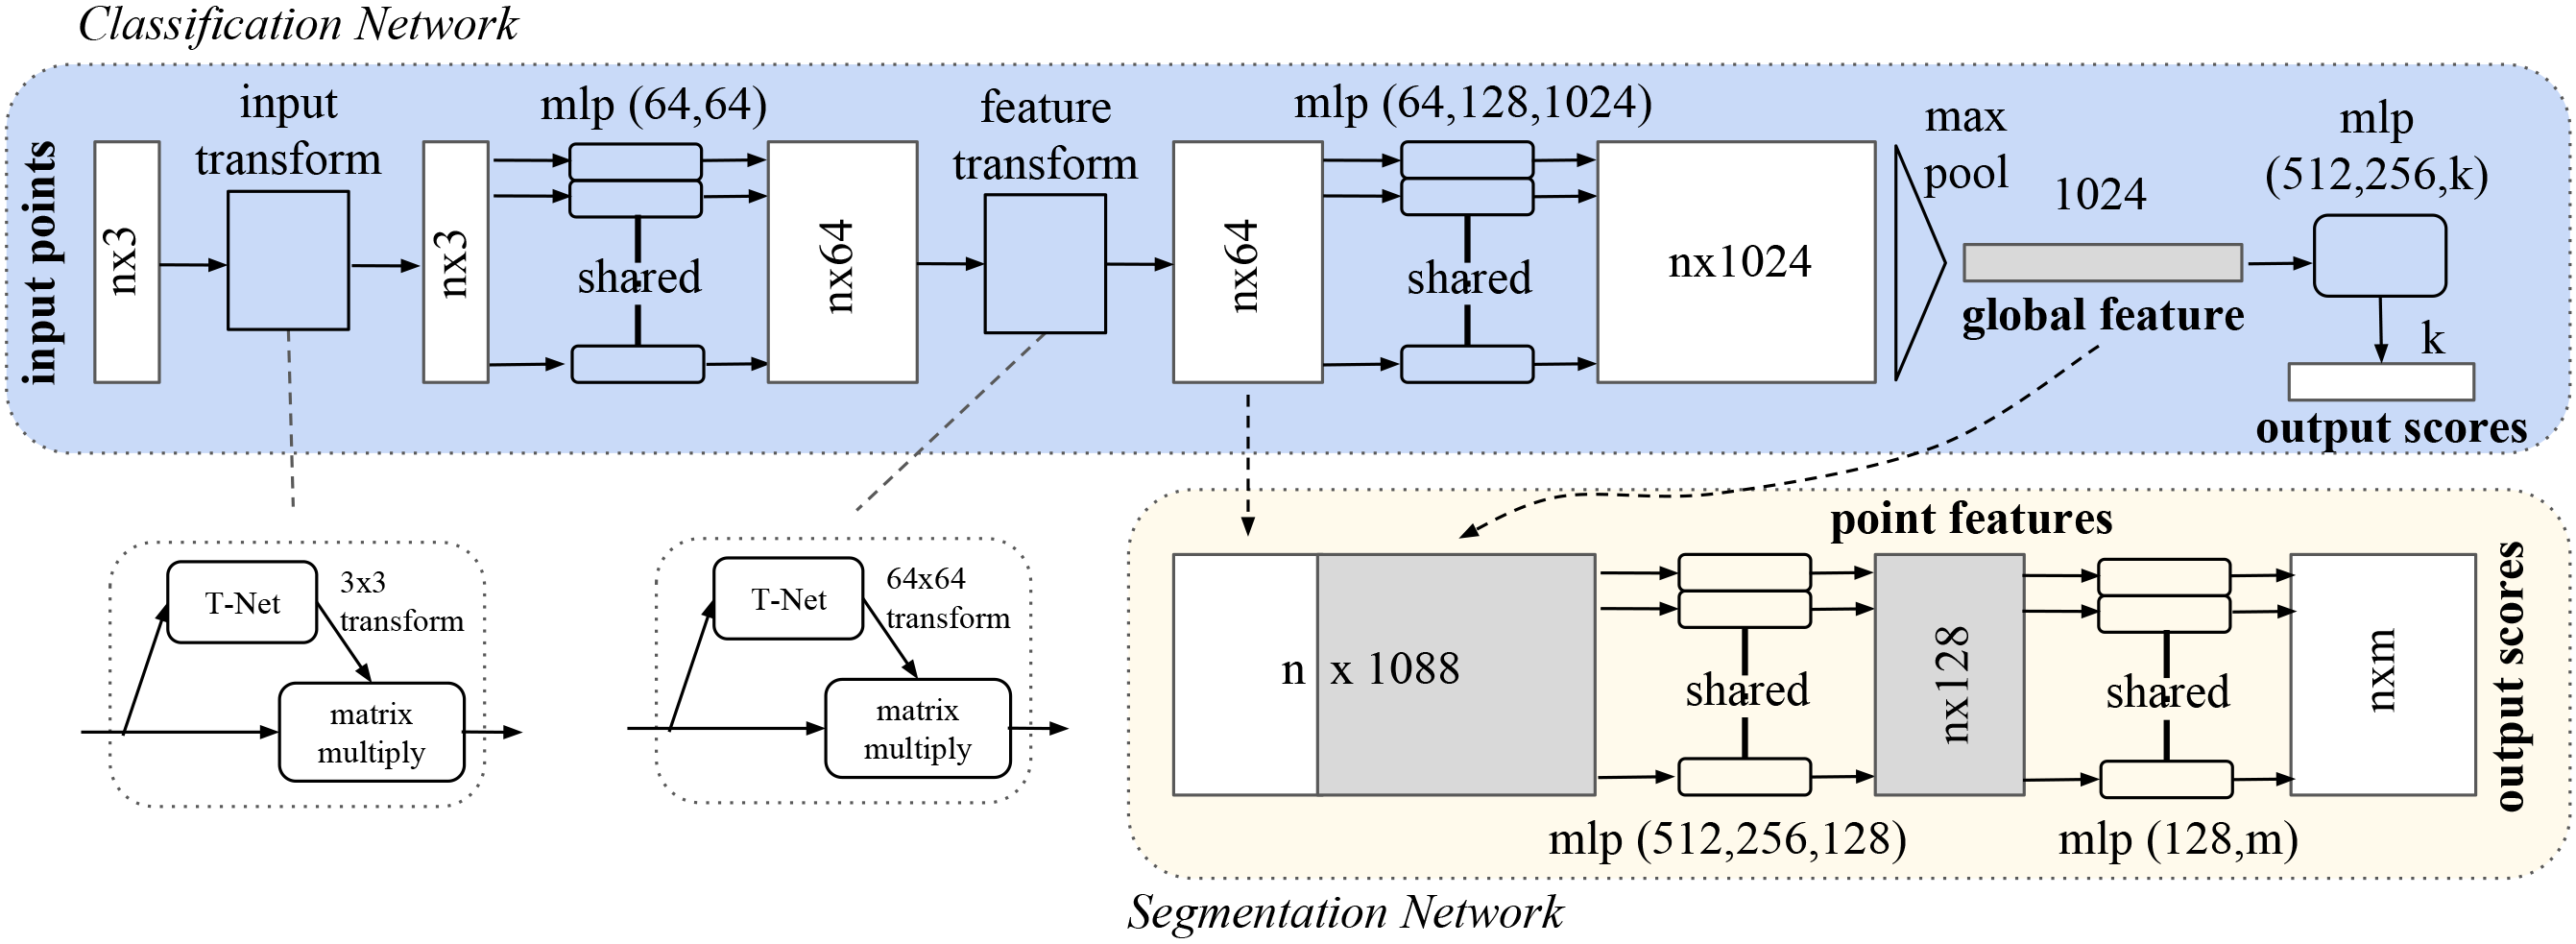
\includegraphics{/img/deep-learning/pointnet.png}
  \caption{PointNet 网络结构示意(来自 \cite{DBLP:journals/corr/QiSMG16})}
  \label{fig:pointnet-arch}
\end{figure}

图 \ref{fig:pointnet-arch} 显示了原论文的网络结构。